\documentclass[11pt]{article}

\usepackage[margin=0.75in]{geometry}
\usepackage{indentfirst}
\usepackage{graphicx}
\bibliographystyle{siam}

\title{The generality of self-control}
\author{
  Chen, Kent\\
  \texttt{kentschen}
  \and
  Lee, Rachel\\
  \texttt{reychil}
  \and
  LeRoy, Benjamin\\
  \texttt{benjaminleroy}
  \and
  Liang, Jane\\
  \texttt{janewliang}
  \and
  Udagawa, Hiroto\\
  \texttt{hiroto-udagawa}
}



\begin{document}
\maketitle

\abstract{% tex file for abstract}

\section{Introduction}
	% tex file for introduction

\section{Data}

	\par \indent BART data consists of the average number of tpumps for each balloon, how many explosions of the balloons, and how much money was earned across each trial for each respective participant. There are four different behavioral variables: the average number of pumps for each balloon, the average across each run, the number of exploded balloons, and ultimately the number of total trials. Within each variable, there are three model conditions: events for inflating the balloon (excluding the very last inflation of each trial), the last inflation before an explosion, and the event when the participant cashes out.
	
\section{Methods}

	\subsection{Convolution}
		% tex file for convolution
\par  \indent Our study has an event-related neurological stimulus, not block stimulus which was discussed in class. We predict the hemoglobin response (HR) related to this type of neurological stimulus, since the methods in class were much better for block stimulus. Moreover our stimulus (as is the case in event-related stimulus studies) wasn't evenly split. We developed a few other functions to take this into account, and will probably implement one more procedure before the end.

\par  The three approaches we will have explored (the first two already completed) address modeling the HR from the neural stimulus. \textbf{(1)} We first implemented the standard block-stimulus paradigm related \texttt{np.convolve} function (which failed to take into account the non-trivial times of stimulus). Np.convolve utilities FFT (Fast Fourier Transforms). \textbf{(2)} Next, we developed a function that doesn't utilize FFT, but allows for dis-continuous events of stimulus (discontinuous, being non-uniform stimulus timing). We used a continuous HR function to model the response (whereas \texttt{np.convolve} uses a discrete HR function).\textbf{(3)} Our next project (\textit{which really should be included in the "Future plans" section}) is to utilize the strength of FFT by splitting up the time into 60 milliseconds intervals (a very small time metric), and then uses \texttt{np.convolve} and some rounding of the stimulus response occurrences to get another candidate for the Hemoglobin response related to the neurological stimulus. This procedure would use the strength of FFT, and wouldn't be hurt by assumptions of time since the HR model isn't super precise and there is a good amount of variance.
    
\par   For \textbf{(2)} and \textbf{(3)} we have to scale back down to the image capturing time frame (2 seconds) [Figure \ref{fig:convolution}].


\begin{figure}[ht]
\centering
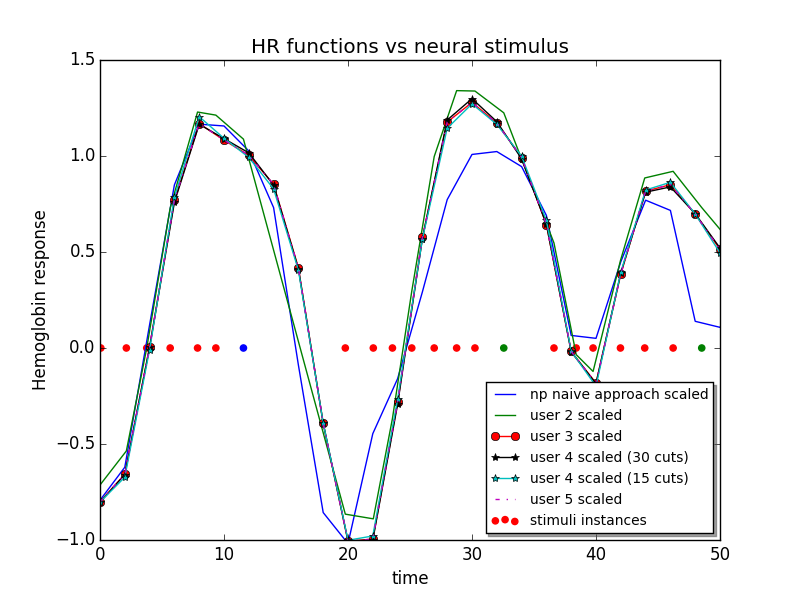
\includegraphics[scale=0.5]{images/convolution_vs_neural_stimulus} 
\caption{Different convolution function vs the Nueral stimulus}
\label{fig:convolution}
\end{figure}


<<<<<<< HEAD
	
=======
>>>>>>> 151a80b3392ce18e09dd52cad2a0b6c2d84503de
	\subsection{Smoothing}
	
		% tex file for smoothing
\par \indent Due to the inherently random nature of human subjects and their movements, a certain level of smoothing must be performed on the spatial dataset. That way, the ‘noisy’ data can be cast off from the data that actually represents significant changes in blood flow in the brain. By doing so, researchers and anyone else investigating the data will be able to distinguish between non-brain scans versus actual brain scans. Each voxel of the brain is represented by a measure of blood flow intensity, and so a series of steps must be taken so that the data is correctly convolved to most closely and accurately depict what was happening at a certain point in the brain at a certain time. After researching quite extensively, we decided to use convolution involving a Gaussian kernel in order to smooth the three dimensional data. Originally, we were going to try and write a smoothing function from scratch, by implementing a rudimentary average-over-neighbors method. However, discussion with mentors lead us to the scipy module \texttt{ndimage.filters} that has a function to performs a Gaussian filter on n-dimensional data. This was exactly what we needed so rather than reinventing the wheel, we will be smoothing the data with this module.

		
	\subsection{Linear Regression}
	
		% tex file for regression
\par \indent A simple and straightforward way to model the voxel time courses is to perform simple and multiple linear regression. As a first attempt, we implemented and performed simple regression on a single subject's 4-dimensional array of voxels against the convolved time course, such that every voxel had an intercept and a coefficient corresponding to the convolved time course. However, examining the effects of the BART experiment conditions on voxel blood flow is also of interest. Thus, we turned to a more sophisticated multiple linear regression model that includes the conditions as dummy variable predictors. In either scenario, we created a design matrix $X$ with the number of rows equal to the number of observed times and the number of rows is equal to the number of predictors. Then, using matrix algebra, we found the matrix of coefficients $\beta$ by calculating $\beta = (X X^T)^{-1} X^T Y$, where $Y$ is the 4-dimensional array of the subject's voxels transformed into two-dimensional space. To do this, we essentially flattened out the first three dimensions (which indicate spatial positions) into a single dimension, while keeping the fourth dimension (time) the same. The resulting $\beta$ was transformed into a three-dimensional array to maintain the spatial relationships of the voxels. 

\par To consider the strength of the effects of these predictors, we looked at t-tests of the corresponding estimated coefficients for each voxel, as discussed under \textit{"Hypothesis Testing"}. Neither of these models, based on our current convolution methods, was very fruitful. 


		
	\subsection{Hypothesis Testing}
	
		% tex file for hypothesis
\par \indent We created our simple linear regression model not necessarily for prediction but rather to understand the relationship between the voxels in a subject's brain and the convolved time course. In order to measure the strength of the relationship between these two measurements, we ran a hypothesis test on the coefficient of the linear regression model.
	\par In our case, we ran a t-test on the $\beta_1$ coefficient of the model with the null hypothesis that $\beta_1=0$ and the alternative hypothesis that $\beta \neq 0$. Since there is a linear model associated with each voxel in a subject’s image, we have a single t-statistic associated to each voxel in our simple linear regression case. Once we had obtained the t-statistic, we compared this value across voxels in two ways. First, we simply compared this value across voxels in a subject. In this case, we took into account the sign of the t-statistic in our analysis. Second, we converted this t-statistic to a p-value, in which case the sign of the t-value will become irrelevant and we compared across voxels without taking into account this sign.  We also developed functions to create t-statistics for multiple feature linear regression. 
	\par \indent Now that we created a method to compare the voxels within a single subject, we next examined our results for the same voxels across subjects. Our initial step was to aggregate the t-statistic data between all subjects for each voxel. This allowed us to decrease the variability of the fit on each voxel and detect a more clear signal. 
	\par \indent In order to do this, we ran the hypothesis test as stated above on all 24 subjects of the study. Then per voxel, we took the simple average of these values. An issue with our data was the presence of empty space that the scanner detected that is not directly part of the brain. In order to account for this, we took the mask data of the brain and ‘cut out’ the parts of the images that were not relevant. 

		
	\subsection{Principal Components Analysis}
	
		\par \indent To perform Principal Components Analysis (PCA), we first considered the method outlined by the guide posted on the class website. Using matrix algebra, we were able to compute principal components by finding orthogonal projections (the shortest distance between points). which has the advantage of projecting the original data so that the predictors are independent. 
\par After consulting with J.B. Poline in lecture, we took a new approach to PCA by implementing the Singular Value Decomposition (SVD) method for 4-dimensional data reshaped to 2-dimensional space. The SVD method is considerably more computationally efficient. With our large number predictors (the time intervals), the original 2-dimensional matrix may be too large to interpret or study because there would be too many correlations to look at. To analyze the data in a more meaningful form, we were able to use PCA to reduce the number of important variables to a few, interpretable linear combinations of our dataset. Though the dimensions of the dataset did not change, we were able to make our dataset easier to explore and visualize. For example, with the help of eigenvectors and eigenvalues, PCA allowed us to focus on the components with the most explained variance. 

		
	\subsection{Time Series Analysis}
	
		% tex file for time series
\par \indent Cohen's paper \cite{CohenSelfControl} discusses analyzing the 
data with time series using FILM (FMRIBs Improved Linear Model). While we are 
not familiar with the FILM method, we did try modeling individual voxels in 
the framework of an autoregressive integrated moving average (ARIMA) process. 
We focused only on a single voxel from the first subject, but the method 
could easily be extended to additional or aggregate voxels. Let $\{Y_t\}$ be 
a single volume's value at time $t$ and assume that the $d$th difference 
$W_t = \nabla^d Y_t$ is weakly stationary, defined to be when $W_t$ has a 
constant mean function and autocovariance dependent only on lag $k$ and not 
time $t$. Then we can try to model $W_t$ as a linear combination of $p$ 
autoregressive terms (or the number of most recent values to include) and $q$ 
moving average terms (the number of lags to include for the white noise error 
terms): 
$$W_t = \phi_1 W_{t-1} + \phi_2 W_{t-2} + ... + \phi_p W_{t-p} + e_t - 
\theta_1 e_{t-1} - \theta_2 e_{t-2} - ... - \theta_q e_{t-q}.$$

\par White noise is defined as a sequence of independent, identically 
distributed random variables. In order to fit an ARIMA process, the three 
orders $p$, $d$, and $q$ must be first be specified, and the the associated 
coefficients estimated. We used a combination of visual inspection and 
quantitative methods to specify the ARIMA orders, and then used the maximum 
likelihood method to estimate parameters. 

		
\section{Results}
		
	\subsection{Linear Regression Results}
	
		% tex file for regression results

\par To develop linear models, we looked at the HR from the neural response 
as a single feature and used multiple regression to take into account the 3 
different types of stimulus (pump, explode, cash-out) to see if the 
separation of these stimuli can better describe the response. Specifically, 
this allows for the prediction of different amplitudes for each type of 
stimulus's HR function in linear regression. The predictive power of these 
models was not very good [Figure \ref{fig:fit_vs_act}] [Figure \ref
{fig:all_cond_time}]. 

\begin{figure}[ht]
\centering
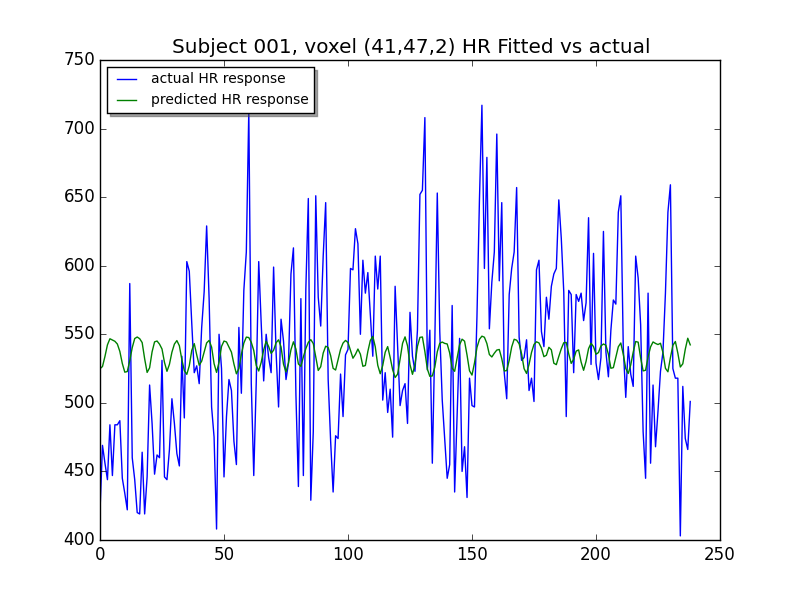
\includegraphics[scale=.5]{images/fitted_vs_actual_mult_regression}
\caption{Fitted vs observed HR based on regressions.}
\label{fig:fit_vs_act}
\end{figure}
  
\begin{figure}[ht]
\centering
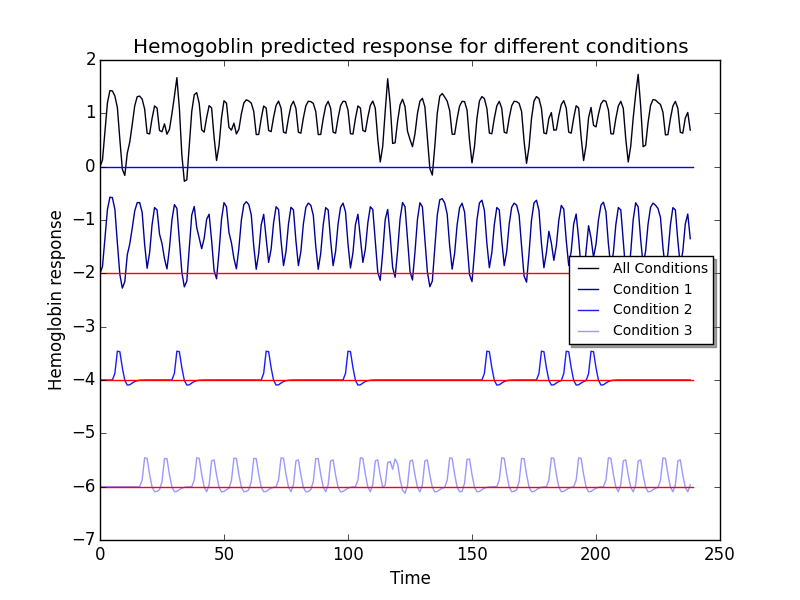
\includegraphics[scale=.5]{images/all_cond_time}  
\caption{Plotting all predicted HR for conditions.}
\label{fig:all_cond_time}
\end{figure}


As we also obtained $\beta$ values (coefficients) from the linear regression 
models, we looked at the 3-dimensional reports of the $\beta$ values, a less 
rigorous analysis than hypothesis testing with t-statistics [Figure \ref
{fig:con1_beta_brain}]. 

\begin{figure}[ht]
\centering
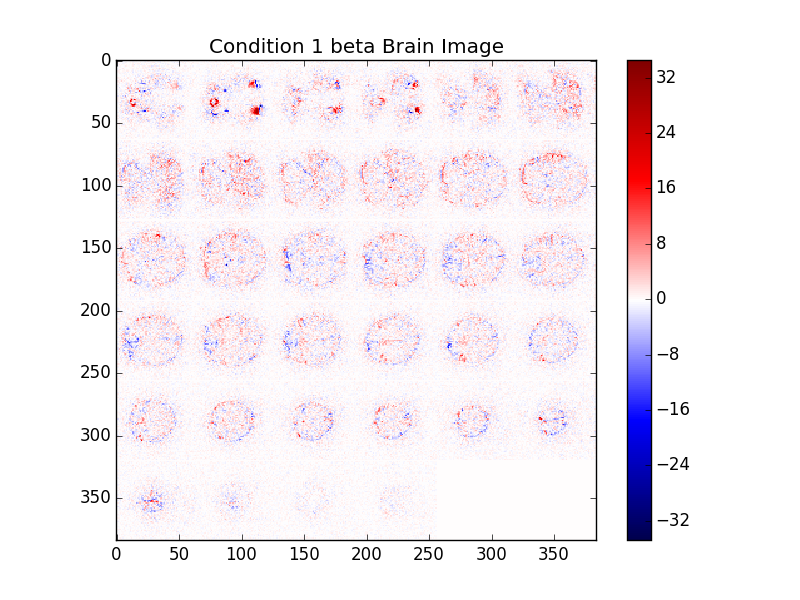
\includegraphics[scale=.5]{images/mr_cond1_beta_brain}    
\caption{$\beta$ values for condition 1, subject 001.}
\label{fig:con1_beta_brain}
\end{figure}


In the future we will include more features to expand beyond information from 
the neural stimulus (see \textit{Discussion of Future Work}).

		
		
	\subsection{Hypothesis Testing Results}
	
		% tex file for hypothesis testing results
\par \indent The results of our simple linear regression t-statistic comparisons across subjects are shown in [Figure \ref{fig:mask}]. We can see each slice of the brain from top to bottom in each section of the image. The blue areas shows parts of the brain that had a negative t-statistic while the red parts of the image shows parts of the brain that had a positive t-statistic.

\begin{figure}[ht]
\centering
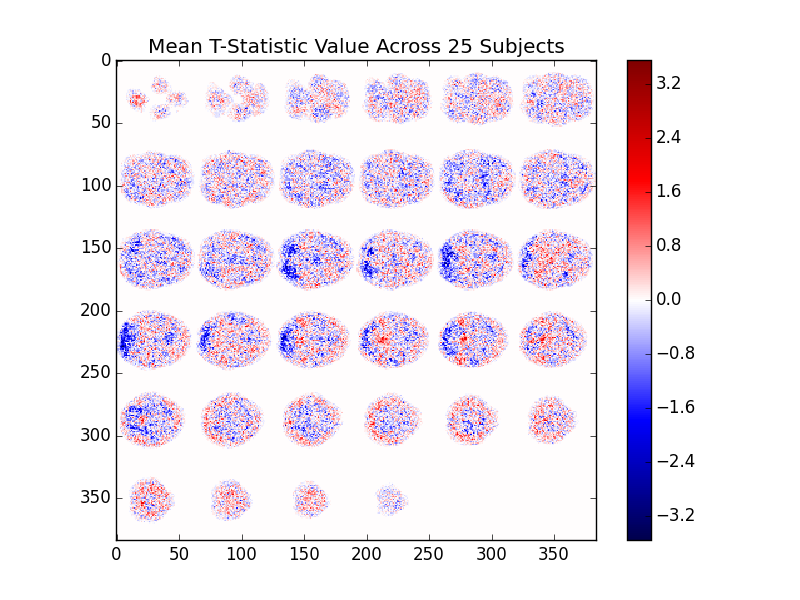
\includegraphics[scale=0.5]{images/hypothesis_testing}  
\caption{Across-subject mean of t-Statistic per voxel.}
\label{fig:mask}
\end{figure}

\par The parts of the image that were cut out by the mask are white so we can more clearly see the contrast in our results. Based on a cursory look at this image, we can see a pattern of dark blue areas in the left middle parts of the brain, and area of dark red in the center middle parts parts of the brain. 



		
	\subsection{Time Series Analysis Results}
	
		\par \indent We considered only a single voxel from the first subject. To specify the orders $p$, $d$, and $q$ for an ARIMA process, we first checked for stationarity by considering the mean function and autocovariance. Visual inspection suggested that the mean function was nonconstant, and additional histograms and quantile-quantile plots suggested a slight skewness with a long right tail. We then corrected the skewness using a log transformation, deemed appropriate by the Box-Cox method. The log-transformed data still exhibited a non-constant mean, so we considered using the first difference (i.e. $W_t = Y_t - Y_{t-1}$). The first difference appeared to be much more reasonably stationary. So, we took $d=1$. 
\par Having specified the order for $d$, we turned to the problem of specifying $p$ and $q$. We used a combination of visually inspecting the autocorrelation and partial autocorrelation plots of the first difference, and looking at the AIC and BIC computed from a grid of possible models. The latter method suggested specifying $p=1$ and $q=1$ (based on either the AIC or the BIC), which was also supported by the visual inspections. 
\par We estimated the parameters for an ARIMA(1,1,1) model using the exact maximum likelihood estimator via Kalman filter. The residuals appear to be normally distributed, and its autocorrelation and partial autocorrelation plots also do not raise any red flags. Furthermore, when visually comparing the fitted time series to the true observed data, the ARIMA process seems to approximate the observed data much better than the linear regression models. While more work, such as developing more robust methods to assess fit and considering the problem of modeling multiple voxels across multiple subjects, is clearly needed, time series analysis presents a promising direction for further investigation. 
\par In particular, we may be able to forecast future observations based on previous ones. As an example we modeled an ARIMA(1,1,1) process based on the first half of the observations for a single voxel. This process was then used to forecast the second half of the observations. A comparison between the true observations and the forecasted predictions is shown in Figure \ref{fig:tsa-preds}. While the forecasted observations look reasonable for approximating the true values, more quantitative metrics for assessing performance need to be implemented. 
\begin{figure}[ht]
\centering
\includegraphics[]{images/tsa-preds}
\label{fig:tsa-preds}
\caption{Forecasting the second half of observations based on the first half.}
\end{figure}


		
\section{Discussion}
	
	\subsection{Discussion of Results}
		
		% tex file for discussion
\par \indent While very much still a work in progress, our analysis thus far includes methods for both data processing and modeling voxel time courses. Prior to doing any serious analysis, we had to smooth the data spatially for each subject and also generate a reasonable convolved time course based on event-related neurological stimuli with non-constant intervals. A basic but nevertheless important model to consider is linear regression. We implemented both simple and multiple regression models at the individual subject level, and performed hypothesis testing on the resulting coefficients for each voxel (and event condition, in the multiple regression case). Finally, we explored some additional methods that may be of interest or use moving forward, including principal components analysis and modeling individual volumes as a time series. 

		
	\subsection{Discussion of Future Work}
	
		% tex file for future discussion
\par \indent To extend our work on multiple linear regression, we will explore methods to account for more of the noise in our data, such as linear drift and discrete cosine transforms for general trends (similar to Fourier series as extra features). We will also be looking into (as long as this is not corrected with pre-processing from out mentors) realignment of scans to correct for the time it takes to scan each voxel compared to the start of the scan. One approach to correct the time shift of when the voxels were actually scanned is to perform resampling techniques.

\par Almost all of our currently implemented methods are designed to handle each subject's data individually. However, we would like to take advantage of all 24 subjects, and would like to explore procedures for comparing results across subjects or aggregating subject data together. 

\par One major concern for hypothesis testing and working with the estimated coefficients from linear modeling is the issue of multiple comparisons. This may be as simple as utilizing a Bonferroni correction, but we can also consider permutation tests or more sophisticated approaches (random fields, Benjamini-Hoffberg, etc). 

\par More quantitative and robust indicators for validating time series models should be implemented. One possibility is to simulate a null process by permuting the phases of the voxel’s time course after performing a Fourier transform, and then transforming the permuted data back to the original space. This way, the data is permuted but maintains the original correlated structure. We can then fit the same ARIMA model to the permuted process and examine how much, if at all, the ARIMA process fitted to the observed data makes improvements over the null case. Generating confidence intervals for the parameter estimates and forecasting future observations may also be of interest. 

		

\bibliography{project}

\end{document}
